\section{Event System}
\label{design:internalcomm}

In \autoref{design:communication} we mentioned that we need a way to provide the user with updates during the long running bootstrapping process.
In order to do this, we introduced event plugins in \autoref{design:plugins} that would allow us to react to events in the bootware.
Now, we will describe the event system that will be used to distribute these events.
Note that this event system is not a core part of the bootware functionality and that the bootware can function completely without it.
It just allows us to access state information of the bootware core and the plugins in a more fine grained way if we need it.

Ideally, we want a central location where we can access all events generated throughout the bootstrapping process.
These events could include events generated by the bootware core, as well as by other plugins.
For example, we might like to receive an event when the process of deploying a new provisioning engine is started.
This would be an event generated by the bootware core when it receives a corresponding deploy request.
During this request execution, multiple plugins would be called to deploy the provisioning engine.
We might also like to receive events during the execution of those plugins.
For example, when a resource plugin creates a cloud resource, it could generate an event when it successfully authenticated with the cloud provider, another event when it started the creation of a VM, and a final event when the VM is ready for use.
We could consume all these event with an event plugin and use them to inform the user of the bootstrapping progress, or log them to a text file.

These events could be triggered by the bootware core or by any plugin, but plugins should be completely independent from each other.
Because an event plugin does not know about other plugins, it can not listen for events at other plugins directly.
The only known constant to an event plugin is the bootware core.
Therefore, we need an event system which allows for loosely coupled communication between the bootware core and the plugins, where plugins can register their interest for certain events with the core and also publish their own events to the core for other plugins to consume.
This essentially describes the publish-subscribe pattern~\autocite{pubsub}.

\subsection{Publish Subscribe Pattern}

The \nom{publish-subscribe pattern}{PubSub} is a messaging pattern that consists of three types of participant: An event bus (or message broker), publishers, and subscribers.
The event bus sits at the center of the communication.
It receives messages from publishers and distributes them to all subscribers that have voiced their interest in messages of a certain type by subscribing at the event bus~\autocite{pubsub}.
Using this pattern, we would create an event bus at the bootware core, and plugins, as well as other parts of the core, could subscribe at this event bus and also publish messages through this event bus.

\begin{figure}[!htbp]
	\centering
	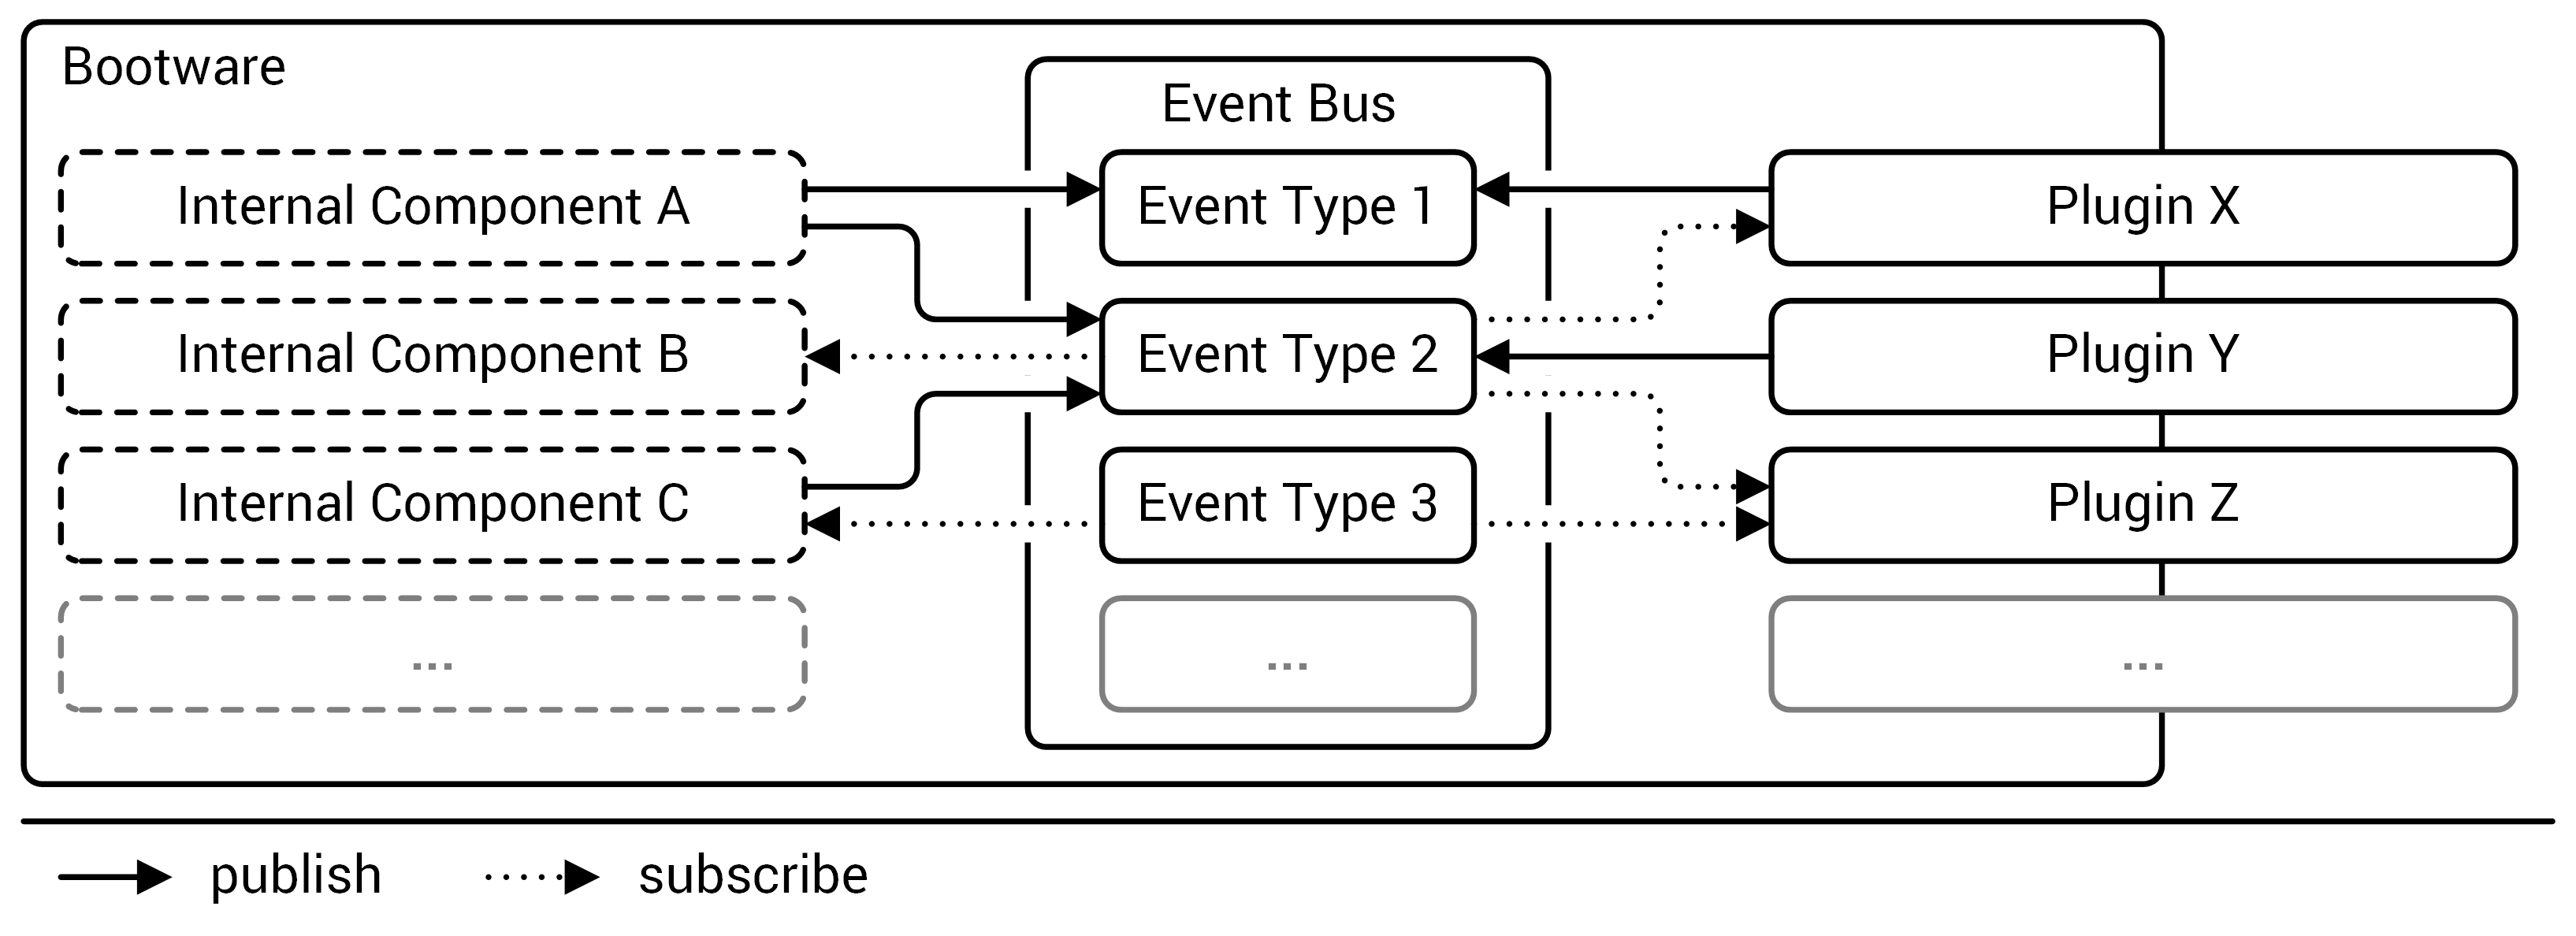
\includegraphics[resolution=600]{design/assets/pubsub}
	\caption{Bootware internal communication with PubSub pattern.}
	\label{image:pubsub}
\end{figure}

\subsection{Event Types}

When using PubSub and events to communicate, it is usually a good idea to not only use one type of event, but many different types.
Using different kinds of event allows us to subscribe only to specific events or react differently based on the event type.
But what if we want to react to each event type in the same way, for example for logging purposes?
Now, many different event types complicate things more.
This is where event hierarchies become useful.
At the core of an event hierarchy is a single base event.
By extending and refining this base event, other, more specific event types can be created, which again can be used as base type for even more specific events.
This allows us to create a fine grained hierarchy of events and also enables us to subscribe to particular sub sets of this hierarchy.
This makes event handling much easier because we can now just react to the parent event if we do not need to distinguish between different event types for a particular task.

A second mechanism to differentiate between events is some sort of severity value that each event contains.
Many events will be published in an event system, but not all of them might be of the same importance.
The majority might be of low value while a few events might be very important.
For example, for logging purposes we might not be interested in every event, but only warnings and errors.
By adding a severity attribute to the base event type, all events could be categorized in different severity groups and filtered accordingly if needed.
As we can see, we might benefit from a well thought-out event hierarchy.

\vspace*{\baselineskip}
\begingroup
	\centering
	\captionsetup{type=figure}
	\begin{description}
		\item[BaseEvent] on which all other events are based
		\begin{description}
			\item[CoreEvent] published by the bootware core
			\begin{description}
				\item[PluginManagerEvent] for loading and unloading plugins
				\begin{description}
					\item[PluginLoadEvent] could be info, success, warning, or error
					\item[PluginUnloadEvent] could be info, success, warning, or error
					\item[\ldots] ~
				\end{description}
				\item[\ldots] ~
			\end{description}
		\end{description}
		\begin{description}
			\item[PluginEvent] published by a plugin
			\begin{description}
				\item[ResourcePluginEvent] contains further child events defined by plugin
				\item[CommunicationPluginEvent] contains further child events defined by plugin
				\item[ApplicationPluginEvent] contains further child events defined by plugin
				\item[EventPluginEvent] contains further child events defined by plugin
				\item[\ldots] ~
			\end{description}
		\end{description}
	\end{description}
	\caption{Exemplary event hierarchy.}
	\label{figure:eventhierarchy}
\endgroup

\autoref{figure:eventhierarchy} shows an exemplary event hierarchy for the bootware.
As we can see, every event is based on the BaseEvent, shown at the top.
Events can be further divided into core events that are published by the bootware core and plugin events that are published by plugins.
Core events contain events from the various core components of the bootware, for example the plugin manager.
The plugin manager events are further divided into events for certain operations that can also have different severity values (e.g.: info, success, warning, and error).
Plugin events are divided by plugin types.
Different plugins can also add further child events to these event types.
